\documentclass[a4paper]{article}
\usepackage[14pt]{extsizes} 
\usepackage[T2A]{fontenc}
\usepackage[utf8]{inputenc}
\usepackage{natbib}
\usepackage{graphicx}
\usepackage{amsmath}
\usepackage[english]{babel}
\usepackage{fontspec}
\usepackage{amsmath,amsfonts,amssymb,amsthm,mathtools,mathrsfs}
\usepackage{icomma}
\usepackage{fullpage}
\usepackage{ulem}
\usepackage{eufrak}
\usepackage{setspace}
\usepackage{listings}
\usepackage{indentfirst}
\usepackage[left=2cm,right=1.5cm,top=2cm,bottom=2cm]{geometry}
\usepackage{xcolor}
\usepackage{float}
\usepackage{csquotes}

\setmainfont[Ligatures={TeX,Historic}]{Times New Roman}
\setlength{\parindent}{5ex}
\setlength{\parskip}{1em}
\renewcommand{\baselinestretch}{1}

\graphicspath{{images/}}

\definecolor{buzzlightyear}{HTML}{8757A5}
\definecolor{grass}{HTML}{738D06}
\definecolor{literal}{HTML}{F18A2B}
\definecolor{commentcolor}{HTML}{8E908B}

\lstdefinestyle{habrstyle}{
    backgroundcolor=\color{white},   
    commentstyle=\color{commentcolor},
    keywordstyle=\bfseries\color{buzzlightyear},
    numberstyle=\tiny\color{commentcolor},
    stringstyle=\color{grass},
    basicstyle=\ttfamily\footnotesize,
    breakatwhitespace=false,         
    breaklines=true,                 
    captionpos=b,                    
    keepspaces=true,                 
    numbers=left,                    
    numbersep=5pt,                  
    showspaces=false,                
    showstringspaces=false,
    showtabs=false,                  
    tabsize=4
}

\lstset{style=habrstyle}

\begin{document}

    % FIRST PAGE
    \begin{center}
        \begin{center}
        \hfill \break
        \normalsize{Санкт-Петербургский государственный политехнический}\\
        \normalsize{университет Петра Великого}\\
        \hfill \break
        \normalsize{\textbf{Высшая школа интеллектуальных систем и}}\\ 
        \normalsize{\textbf{суперкомпьютерных технологий}}\\ 
        \hfill \break
        \hfill \break
        \hfill \break
        \normalsize{Лабораторная работа}\\
        \hfill \break
        \hfill \break
        \normalsize{\LARGE Дискретное косинусное преобразование}\\
        \end{center}
        \hfill \break
        \hfill \break
        \hfill \break
        \hfill \break
        \hfill \break
        \hfill \break
        \hfill \break
        \hfill \break
        \hfill \break
        \hfill \break
        \begin{flushright}
            \normalsize{Работу выполнил студент}\\
            \normalsize{3-го курса, группа 3530901/80201}\\
            \normalsize{Сахибгареев Рамис Ринатович}\\
            \hfill \break
            \normalsize{Преподаватель:}\\
            \normalsize{Богач Наталья Владимировна}\\
        \end{flushright}
        \hfill \break
        \hfill \break
        \hfill \break
        \hfill \break
        \begin{center} Санкт-Петербург 2021 \end{center}
        \thispagestyle{empty}
    \end{center}
    % FIRST PAGE [END]
    
    \newpage
        \tableofcontents
    
    \newpage
         \listoffigures
    
    \newpage
         \lstlistoflistings   
     
    % START START START START START
    \newpage
        \section{Part 1: Amplitude effectiveness comparison}
        
        In this part we need to compare linalg and matrix ways of estimate amplitudes of DCT.
        
        Firstly, lets define some helper function, analysis functions itself and analyzed wave.
        
        \begin{lstlisting}[language=Python,caption=Functions definition,label={lst:part1_1}]
    from thinkdsp import *
    from scipy.stats import linregress
    import thinkplot
    import numpy as np
    import matplotlib.pyplot as plt
    
    sig = UncorrelatedGaussianNoise()
    wave = sig.make_wave(duration = 1, framerate = 2**14)
    def plot_res(tm, ns, clr='cyan'):
        thinkplot.plot(ns, tm, color=clr)
        
        x = np.log(ns)
        y = np.log(tm)
        t = linregress(x,y)
        slope = t[0]
        
        return slope
    def analyze1(ys, fs, ts):
        args = np.outer(ts, fs)
        M = np.cos(PI2 * args)
        amps = np.linalg.solve(M, ys)
        return amps
    def analyze2(ys, fs, ts):
        args = np.outer(ts, fs)
        M = np.cos(PI2 * args)
        amps = np.dot(M, ys) / 2
        return amps
        \end{lstlisting}
        
        Now we can create a little benchmark, that performs analyze by incriminating length of the wave step by step.
        
        \begin{lstlisting}[language=Python,caption=Benchmark code,label={lst:part1_1}]
    res1 = []
    res2 = []
    ns = 2 ** np.arange(6, 13)
    for n in ns:
        ts = (0.5 + np.arange(n)) / n
        fq = (0.5 + np.arange(n)) / 2
        ys = wave.ys[:n]
        r1 = %timeit -r1 -o analyze1(ys, fq, ts)
        r2 = %timeit -r1 -o analyze1(ys, fq, ts)
        res1.append(r1)
        res2.append(r2)
    
    t1 = [r.best for r in res1]
    t2 = [r.best for r in res2]
    print("first ", plot_res(t1, ns))
    print("second ", plot_res(t2, ns, clr='orange'))
        \end{lstlisting}
        
        \begin{figure}[H]
            \centering
            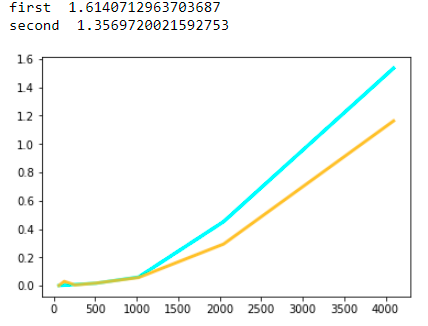
\includegraphics[width=\textwidth]{img/funct_anlz.png}
            \caption{Benchmark result}
            \label{fig:part1_1_1}
        \end{figure}
        
        We can see, that matrix way is much faster, than linear algebra way of estimating DCT amplitude.
        
    \newpage
        \section{Part 2: Sound compression algorithm}

        In this part we need to implement simple sound compression algorithm by splitting the signal into the parts and removing near to 0 components from spectrum. Let's define compression algorithm. Compress function removes near 0 components, \texttt{makedctspectrogram} makes DCT spectrogram. 
        
        \begin{lstlisting}[language=Python,caption=Functions definition,label={lst:part1_2}]
    def compress(dct, thresh=1):
        count = 0
        for i, amp in enumerate(dct.amps):
            if np.abs(amp) < thresh:
                dct.hs[i] = 0
                count += 1
                
        n = len(dct.amps)
        return (count, n)
    def make_dct_spectrogram(wave, seg_length):
        window = np.hamming(seg_length)
        i, j = 0, seg_length
        step = seg_length // 2
        spec_map = {}
        while j < len(wave.ys):
            segment = wave.slice(i, j)
            segment.window(window)
            t = (segment.start + segment.end) / 2
            spec_map[t] = segment.make_dct()
            i += step
            j += step
        return Spectrogram(spec_map, seg_length)
        \end{lstlisting}
        
        Let's compress Halzion by YOASOBI. We can see. that its segment has a lot of near 0 components, that can be removed.
        
        \begin{lstlisting}[language=Python,caption=Reading the waver,label={lst:part1_2}]
    wave = read_wave('sound/halzion.wav')
        segment = wave.segment(start=20, duration=0.1)
        segment.make_spectrum().plot()
        wave.make_audio()
        \end{lstlisting}
        
        \begin{figure}[H]
            \centering
            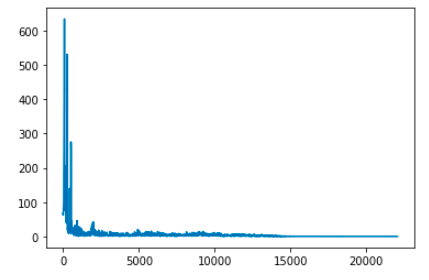
\includegraphics[width=\textwidth]{img/halzion_spec.png}
            \caption{Halzion's segment spectrogram}
            \label{fig:part1_1_2}
        \end{figure}
        
        By splitting this song into the segments of 512 elements and removing every component with amplitude less than a 0 we've got 67 percent spectrum size reduction.D
            
        \begin{lstlisting}[language=Python,caption={Compression of the wave},label={lst:sawtooth_def}]
    spectrogram = make_dct_spectrogram(wave, seg_length=512)
    total = 0;
    rem = 0;
    for t, dct in spectrogram.spec_map.items():
        cnt, n = compress(dct, thresh=1)
        total += n;
        rem += cnt;
    print("removed", rem, "of", total, "percent", rem / total)
        \end{lstlisting}
        
        \begin{figure}[H]
            \centering
            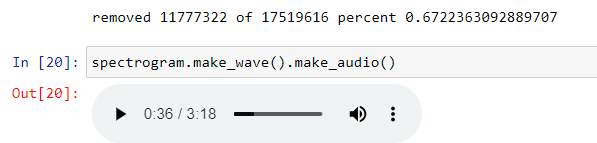
\includegraphics[width=\textwidth]{img/halzion_comp.png}
            \caption{Halzion compression result}
            \label{fig:part1_1_2}
        \end{figure}
        
        By listening the resulting audio I can say, that sound now is unpleasant to hear because of buzzing.
        
    \newpage
        \section{Part 3: Playing with a phace}
            
        In this part we need to investigate a phase effect on the signal perception. 
        
        To do it thiangle signal with frequency of 500 Hz was generated. If we will plot its phases plot we see, that we have a lot of noise on the plot because of aliasing effect. 
        
        \begin{figure}[H]
            \centering
            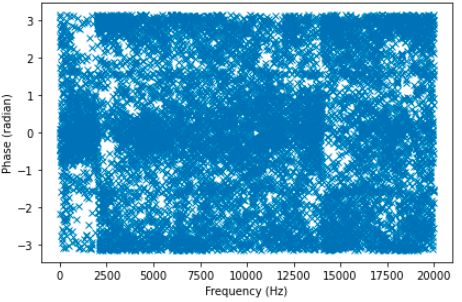
\includegraphics[width=\textwidth]{img/ph1.png}
            \caption{Phases noise}
            \label{fig:als_sqr}
        \end{figure}
        
        We can get rid of this noise by cutting off frequencies with amplitude lower than threshold. The resulting set of plots is next. We can see, that phase increases linearly by its frequency.
            
        \begin{figure}[H]
            \centering
            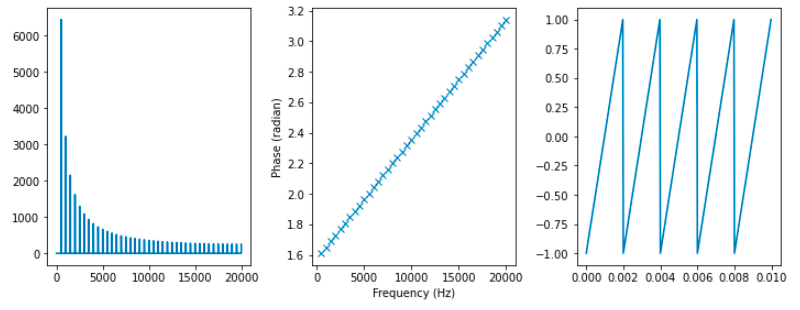
\includegraphics[width=\textwidth]{img/ph2.png}
            \caption{Triangle signal plot set}
            \label{fig:als_sqr}
        \end{figure}
        
        If we set phase of every frequency to 0, we see that signal changed dramatically, but we cannot hear any difference with the original one.
        
        \begin{figure}[H]
            \centering
            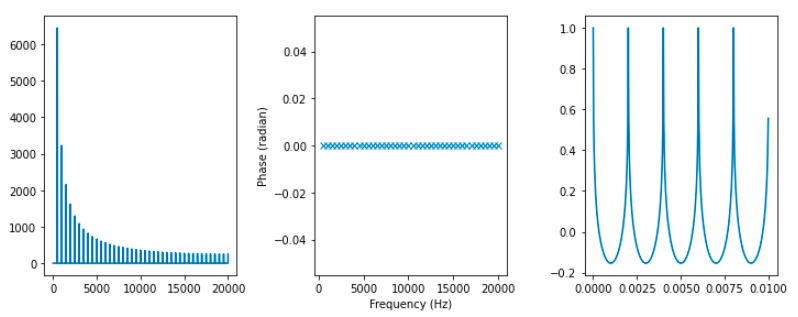
\includegraphics[width=\textwidth]{img/ph3.png}
            \caption{Triangle signal phase = 0}
            \label{fig:als_clr}
        \end{figure}
            
        If we rotate phases by some value, we can see that plots changes a lot too, but again we cannot hear any difference with the original signal.
        
        \begin{figure}[H]
            \centering
            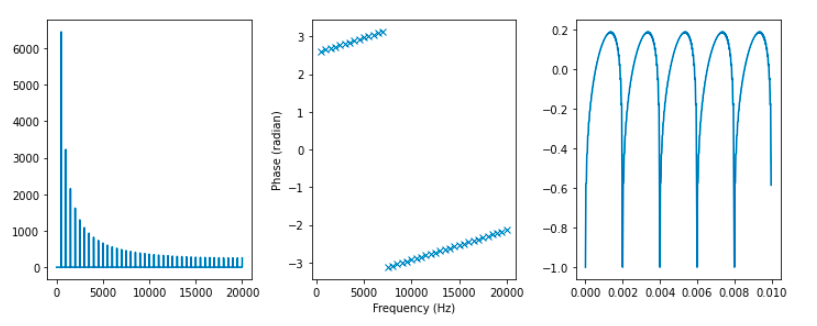
\includegraphics[width=\textwidth]{img/ph4.png}
            \caption{Triangle signal phase rotated}
            \label{fig:als_clr}
        \end{figure}
            
        Lastly, let's set every angle to the random value. We can see, that signal doesn't looks like the triangle one at all, but again we cannot hear any difference.
        
        \begin{figure}[H]
            \centering
            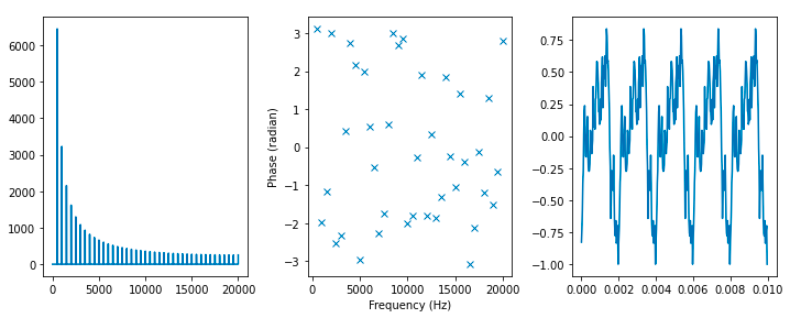
\includegraphics[width=\textwidth]{img/ph5.png}
            \caption{Triangle signal phase = random}
            \label{fig:als_clr}
        \end{figure}
        
        But this happens not to the all signals. If we will use more complex signal like oboe record, we see other things happen.
        
        Let's look at the original signal's plots.
        
        \begin{figure}[H]
            \centering
            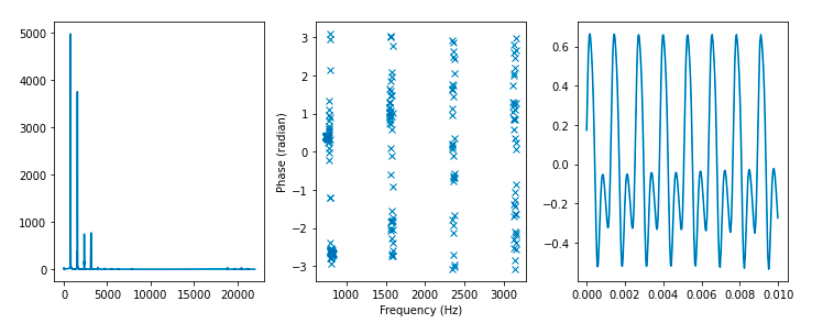
\includegraphics[width=\textwidth]{img/ph6.png}
            \caption{Oboe record plots}
            \label{fig:als_clr}
        \end{figure}
        
        By setting every phase to 0 we won't get the same sound, as it was with triangle sound. Sound changes its volume over the time.
        
        \begin{figure}[H]
            \centering
            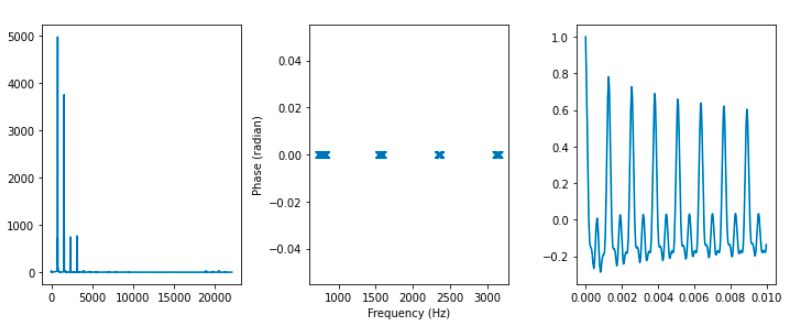
\includegraphics[width=\textwidth]{img/ph7.png}
            \caption{Oboe record phase = 0}
            \label{fig:als_clr}
        \end{figure}
        
        By rotating the signal by some angle we won't get this effect, and plot looks like the original one.
        
        \begin{figure}[H]
            \centering
            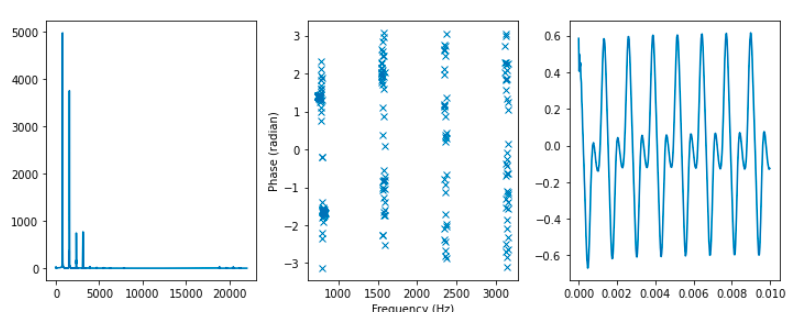
\includegraphics[width=\textwidth]{img/ph8.png}
            \caption{Oboe record phase rotated}
            \label{fig:als_clr}
        \end{figure}
        
        However, randomizing the phases returns this effect. Plot also looks "wrong".
        
        \begin{figure}[H]
            \centering
            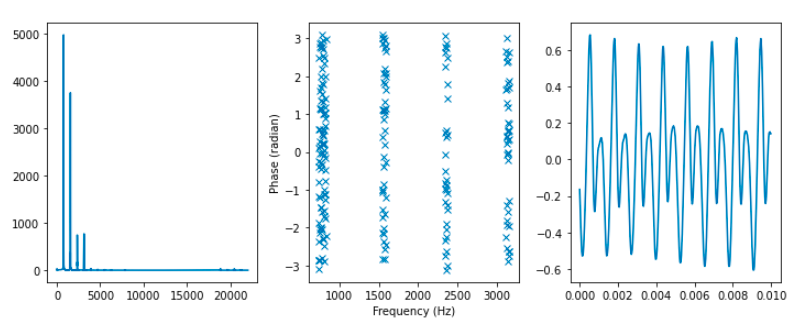
\includegraphics[width=\textwidth]{img/ph9.png}
            \caption{Oboe record phase randomized}
            \label{fig:als_clr}
        \end{figure}
        
        Next, we can apply this method to research a saxophone record. Saxophone spectrum looks like triangle signal, but has a low amplitude base frequency.
        
        \begin{figure}[H]
            \centering
            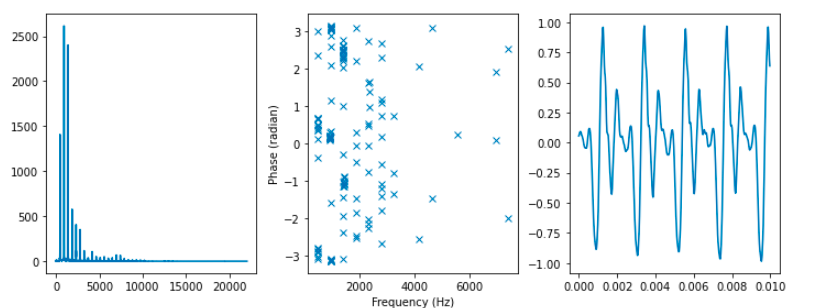
\includegraphics[width=\textwidth]{img/ph10.png}
            \caption{Saxophone record plots}
            \label{fig:als_clr}
        \end{figure}
        
        After hearing its audio after each operation we can say, that saxophone's audios have same behavior as oboe's does.
        Let's remove base frequency from saxophone signal.
        
        \begin{figure}[H]
            \centering
            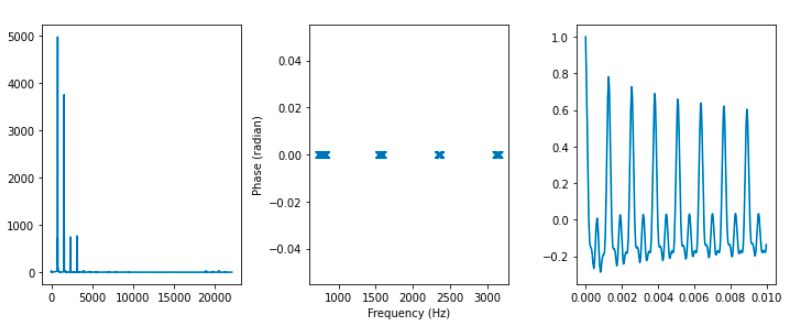
\includegraphics[width=\textwidth]{img/ph7.png}
            \caption{Saxophone record without base frequency}
            \label{fig:als_clr}
        \end{figure}
        
        After hearing its audio we can say, that now it behaves like triangle signal does.
        After all, we can say, that simple signals doesn't changes a lot if their phases are being changed in some way.
        However, more complex signals changes after their phases was changed.
            
    \newpage
        \section{Conclusion}
            We've learned, what is DCT and how we can use it by compressing the signal. Also we've learned different ways of estimating an amplitude of a signal by knowing it's frequencies and benchmarked them. Last, we've learned how phase affects the signal's perception by a human ear.
     
\end{document}
